\documentclass[ngerman]{beamer}
\usetheme{metropolis}

% use \cref instead of autoref, autoref does not work with beamer
\usepackage{cleveref}

% some imports from handout, probably dont need all but whatever
\usepackage[utf8]{inputenc}
\usepackage[T1]{fontenc}   
\usepackage{graphicx}       
\usepackage[german]{babel}
\usepackage{csquotes}     
\usepackage{eurosym}
\usepackage{float}
\usepackage{rotating}
\usepackage{blkarray}
\usepackage{amsmath}
\usepackage{amssymb}
\usepackage{gensymb}
\usepackage{amsthm}
\usepackage{listings}
\usepackage{caption}
\usepackage{subcaption}
\usepackage{interval}


% argmin command
\newcommand{\argmin}[1]{\underset{#1}{\operatorname{arg}\,\operatorname{min}}\;}
% command for euclidean norm
\newcommand{\norm}[1]{\lVert#1\rVert}
% command for lagrangian L (kind of handwritten L)
\newcommand{\Lagr}{\mathcal{L}}

% show current page number in footer
\setbeamertemplate{footline}[frame number]

% No navigation symbols at the slides' bottom
\beamertemplatenavigationsymbolsempty



\title{Support Vector Machines}
\author{André Hopfgartner \& Matthias Rupp}
\begin{document}
	
\begin{frame}[plain]
    \maketitle
\end{frame}

\begin{frame}{Frame Title}
\begin{itemize}
	\item Eine Hard-Margin SVM trennt die Klassen so, dass keine Fehlklassifikationen entstehen. 
	\pause 
	\item Eine Soft-Margin SVM erlaubt einzelne Fehlklassifikationen damit eine mitunter bessere Trennebene gefunden werden kann.
\end{itemize}
	
\end{frame}

\frame{
	\frametitle{A test with images}
	\framesubtitle{subcaption testing with images}
	\begin{minipage}{0.5\textwidth}

		\begin{itemize}
			\item Some 
			\item text 
			\item on left side of slide here..
			\item \cref{fig:intuition_margin} zeigt blabla.
		\end{itemize}
		\pause
	\end{minipage} \hfill
	\begin{minipage}{0.45\textwidth}
	\begin{figure}
		\centering
		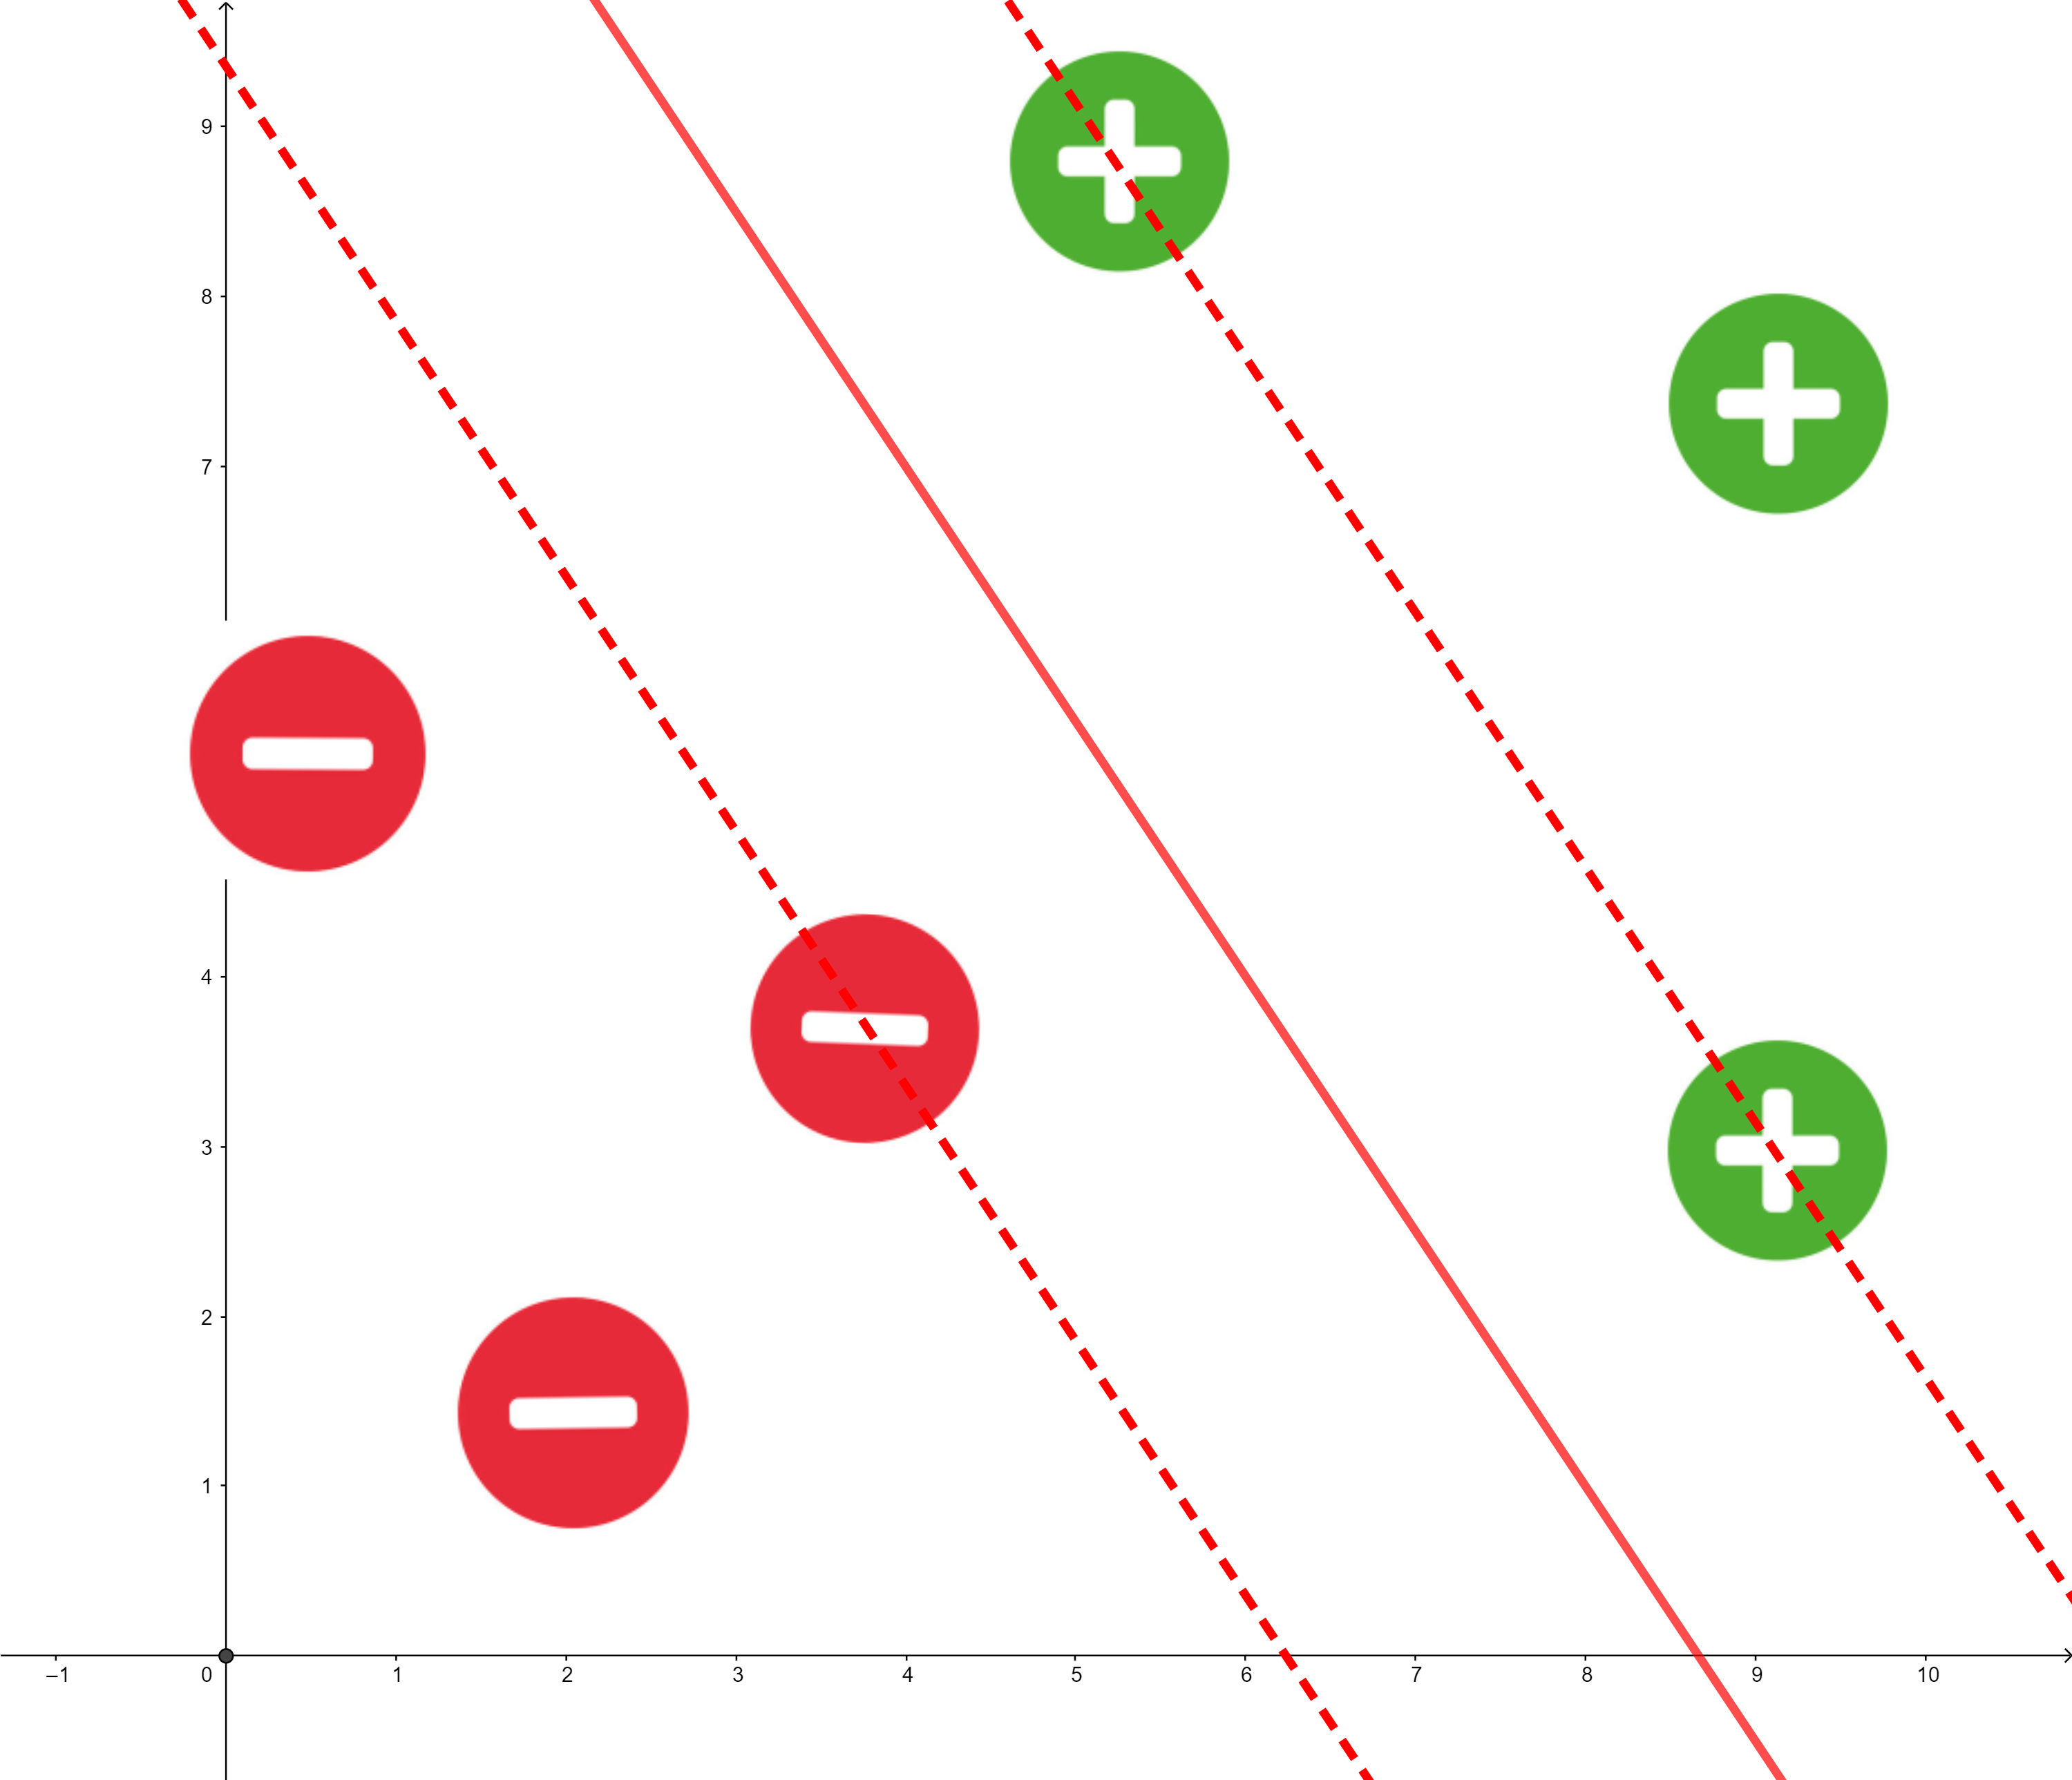
\includegraphics[height=0.9\textwidth]{assets/intuition_big_margin.png}
		\caption{Abhängig von der Lage der Trennebene entstehen schmale (blau) oder breite (rot) Trennbänder. Ziel ist die Maximierung der Breite des Trennbands durch die Ermittlung der optimalen Lage der Trennebene.}
		\label{fig:intuition_margin}
	\end{figure}
	\end{minipage}
}

\begin{frame}
	\begin{subequations} \label{svm_classify1}
		\begin{alignat}{2}
			y = sign(w^{T} x + b)  & \qquad & \text{ gleichbedeutend mit} \\
			w^{T} x + b > 0 & & \text{ für } y = +1\\
			w^{T} x + b < 0 & & \text{ für } y = -1
		\end{alignat}
	\end{subequations}

	In \cref{svm_classify1} wird ..
\end{frame}




\end{document}

